\documentclass{article}

\usepackage[utf8]{inputenc}
\usepackage[a3paper, margin=1in]{geometry}
\usepackage{booktabs}
\usepackage{graphicx}

\title{Data Exercise Notes}
\author{Saksham Kaushal}


\begin{document}
	\maketitle
	
	\section{Photometry}
	\begin{enumerate}
		
		\item \textbf{Do you understand what is changing?} -- using \emph{autocut, colour map, intensity map,} and \emph{colour bar}.
		
		\item \textbf{How can you determine which object is the nova?}
		
		Using multiple images. Nova are transients with their luminosities fading over time, typically few days/weeks. So, looking out for stars with luminosities fading over time would help us determine which object is a nova.
		\(\alpha = 00:44:41.05, \delta = 40:08:36.00\)
		
		\item \textbf{Header contents, position and pixel information}
		
		\begin{table} [h] 
			\centering
			\begin{tabular}[width=\linewidth] {l r r r r r}
				\toprule
				\textbf{file} & \textbf{DATE-OBS} & \textbf{MJD} & \textbf{EXPTIME} & \textbf{AIRMASS} & \textbf{x-axis span} \\
				\midrule
				phot\_00.fits & 2016/07/16 01:54:04.626 & 57585.079220 & 120 & 1.7258910 & 1049--1061 \\
				phot\_01.fits & 2016/07/17 01:57:55.414 & 57586.081891 & 120 & 1.6665240 & 1049--1061 \\
				phot\_02.fits & 2016/07/18 01:43:20.318 & 57587.071763 & 120 & 1.7491860 & 1049--1061 \\
				phot\_03.fits & 2016/07/19 01:36:39.439 & 57588.067123 & 120 & 1.7721150 & 1050--1061 \\
				phot\_04.fits & 2016/07/22 02:34:57.627 & 57591.107611 & 120 & 1.3530670 & 1052--1058 \\
				phot\_05.fits & 2016/07/25 01:29:33.555 & 57594.062194 & 120 & 1.6443790 & 1053--1058 \\
				phot\_06.fits & 2016/07/27 01:35:03.477 & 57596.066012 & 120 & 1.5562500 & 1052--1058 \\
				phot\_07.fits & 2016/08/03 03:15:00.354 & 57603.135421 & 120 & 1.1115970 & 1053--1058 \\
				phot\_08.fits & 2016/08/09 01:19:45.090 & 57609.055383 & 120 & 1.3717510 & 1050--1060 \\
				phot\_09.fits & 2016/08/17 01:26:10.686 & 57617.059846 & 120 & 1.2355820 & 1053--1058 \\
				phot\_10.fits & 2016/08/19 02:09:48.268 & 57619.090142 & 120 & 1.1156090 & 1053--1058 \\
				phot\_11.fits & 2016/08/21 02:53:30.765 & 57621.120495 & 120 & 1.0482370 & --- \\
				phot\_12.fits & 2016/08/27 01:30:12.240 & 57627.062642 & 120 & 1.1306350 & 1053--1057 \\
				phot\_13.fits & 2016/08/29 03:01:21.059 & 57629.125938 & 120 & 1.0244450 & 1054--1057 \\
				phot\_14.fits & 2016/09/06 02:28:01.479 & 57637.102795 & 120 & 1.0250930 & 1054--1057 \\
				phot\_15.fits & 2016/09/13 23:52:30.836 & 57644.994801 & 120 & 1.1904340 & 1054--1056 \\
				phot\_16.fits & 2016/09/24 02:27:20.058 & 57655.102315 & 300 & 1.0329910 & 1053--1056 \\
				phot\_17.fits & 2016/09/28 02:53:32.834 & 57659.120519 & 300 & 1.0706010 & 1054--1056 \\
				\bottomrule
			\end{tabular}
		\end{table}
		GAIN = 1.62, Position = (1055,978) for all entries. 
		
		\item \textbf{Are the number of pixels containing light from the nova (i.e. the point spread function or PSF) the
			same in every image? What two effects could be changing this?}
		
		No. Change in auto-cut value and variations in brightness of background or nova can change the viewed psf.
		
		\item \textbf{Why is it important to do this?} -- enter \emph{exposure time} and \emph{gain} for each observation.
		
		Image of a faint object captured over long exposure time may be brighter than the image of a bright object captured over smaller exposure time. Similarly, high gain would require more photons per data unit. Therefore, for different values of gain too, our perception of bright and faint objects may vary from one image to another. Hence, it is important to account for exposure time and gain for each image.
		
		\item \textbf{Why would it be undesirable to use an aperture that is either too small or too large?}
		
		A very small aperture would lead to loss of signal by discarding useful signal. A large aperture would include a lot of noise. Hence in both cases, signal to noise ratio is decreased, although in different ways. An optimal aperture considers all the signal while discarding maximum possible noise. In aperture photometry, the outer annulus is used to account for calculate average noise value. This value is subtracted from the aperture signal to obtain true signal. If the aperture contains noise (very large aperture) or discards signal (very small aperture), the calculated value will account for smaller than true overall value of signal or signal to noise ratio. 
		
		\item \textbf{Signal to noise ratios for different apertures. How do you decide which aperture is optimal?}
		
		\begin{table} [h]
			\centering
			\begin{tabular} {r r r r r r}
				\toprule
				\textbf{radius} & \textbf{magnitude} &\textbf{mag error} & \textbf{signal} & \textbf{noise} &\textbf{SNR} \\
				\midrule
				6.0 & -8.02378 & 0.00512 & 3656.2 & 1620.0 & 2.257 \\
				10.4 & -8.13224 & 0.00738 & 3629.6 & 1790.2 & 2.0275 \\
				15.5 & -8.15562 & 0.01047 & 3627.2 & 1829.1 & 1.983 \\
				26.5 & -8.16615 & 0.01745 & 3626.2 & 1847.0 & 1.963 \\
				\bottomrule
			\end{tabular}
		\end{table}
		
		Optimal is systematically decided using data count results instead of magnitude results. A rough estimate for better understanding can be performed using table above.
		
		\item \textbf{Do the results you have obtained, by varying the aperture size, vary randomly as you might expect with measurement error?}
		
		No. Results vary in a well defined manner according to the reasons stated above. The errors are not random, and instead depend upon the radius of the aperture. Both small and large apertures are inefficient and an optimum aperture lies in between that range.
		
		\item \textbf{determine the optimal aperture size.}
		
		\begin{table} [h]
			\centering
			\begin{tabular} {l r r r}
				\toprule
				\textbf{aperture (semi-major axis)} & \textbf{mean counts} & \textbf{error in counts} & \textbf{SNR}\\
				\midrule
				3.0 & 36.784 & 0.10739 & 342.527 \\
				4.0 & 26.835 & 0.037792 & 710.071 \\
				5.0 & 19.433 & 0.024469 & 794.189 \\
				6.0 & 14.398 & 0.016884 & 852.760 \\
				7.0 & 11.029 & 0.013013 & 847.537 \\
				8.0 & 8.6644 & 0.011412 & 759.236 \\
				9.0 & 6.9651 & 0.010593 & 657.519 \\
				10.0 & 5.7077 & 0.010112 & 564.448 \\
				11.0 & 4.7566 & 0.0094432 & 503.706 \\
				12.0 & 4.0395 & 0.0089313 & 452.286 \\
				13.0 & 3.4646 & 0.0082037 & 422.322 \\
				14.0 & 2.9852 & 0.0072329 & 412.725 \\
				15.0 & 2.6030 & 0.0066956 & 388.763 \\
				16.0 & 2.2916 & 0.0062298 & 367.845 \\
				17.0 & 2.0352 & 0.0057338 & 354.948 \\
				18.0 & 1.8190 & 0.0054112 & 336.155 \\
				19.0 & 1.6286 & 0.0051199 & 318.092 \\
				20.0 & 1.4728 & 0.0048525 & 303.514 \\
				25.0 & 0.94289 & 0.0039804 & 236.883 \\
				\bottomrule
			\end{tabular}
		\end{table}
		\(r_a=1.5\) and \(r_b=2.0\). SNR = [342.527,710.071,794.189,852.760,847.537,759.236, 657.519, 564.448, 503.706, 452.286, 422.322, 412.725, 388.763, 367.845, 354.948, 336.155, 318.092, 303.514]
		
		\begin{figure}[h]
			\centering
			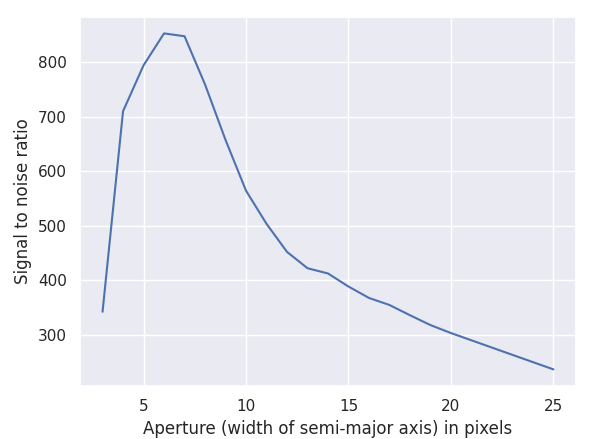
\includegraphics[width=.7\linewidth]{../codes/plots/optimal_aperture_phot_00.png}
		\end{figure}
		
		
		\item \textbf{What would be the effect of changing the aperture size between measurements within the same image?}
		
		Would give inconsistent values of magnitudes for different objects.  
		
		\item \textbf{Optimal apertures for all images.}
		\begin{table}[h]
			\centering
			\begin{tabular} {l r}
				\toprule
				\textbf{file} & \textbf{aperture} \\
				\midrule
				00 & 7.0 \\
				01 & 6.5 \\
				02 & 5.5 \\
				03 & 5.4 \\
				04 & 4.9 \\
				05 & 4.9 \\
				06 & 8.0 \\
				07 & 4.4 \\
				08 & 7.5 \\
				09 & 4.6 \\
				10 & 3.1 \\
				11 & 4.4 \\
				12 & 3.6 \\
				13 & 2.5 \\
				14 & 2.3 \\
				15 & 4.2 \\
				16 & 3.3 \\
				17 & 2.9 \\
				\bottomrule
			\end{tabular}
		\end{table}
		
		\item \textbf{Does the optimal aperture size vary between the images? If so, what causes this?}
		
		Optimal aperture size varies for different images depending upon atmospheric seeing (or the background noise), exposure time, object brightness, etc.
		
		\item \textbf{Why does this approach work?
What problems might be associated with this method?} -- using secondary stars for photometry.
		
		We need to consider only the stars which have been observed to remain static (i.e. not a variable star) over extremely long periods, so that its low photometric uncertainty can be considered reliable for calibration. If such a non-variable star lies in our field of view while observing the science object, the photometry of that object can be calibrated using the nearby secondary standard. Even if the atmospheric conditions are not very favourable, photometry can still be performed if we can safely assume that the extent of unfavourability of conditions is similar for both the objects, which is a reasonable assumption for nearby secondary standards. Secondly, widely separated secondary stars in the field of view can be used to estimate variability in atmospheric extinction across field of view. For faint events, exposure times are long and many of the primary standards appear saturated. Dimmer secondary stars therefore are more helpful in these cases.
		
		 \item \textbf{How can we determine which of the PS1 stars might be suitable to use?}
		
		Vicinity to the nova and comparable brightness. Vicinity would lead to correlating atmospheric extinction values, which would be roughly similar for all, and therefore, easily accounted for. Similar brightness or \emph{spread} of stars would aid the use of same aperture for all standard stars and nova in the image. Also, every secondary star selected should be properly resolved in the image.
		
		\item \textbf{Secondary stars}
		
		ID = [11,2,6,30,10]
		
		\item \textbf{Photometry of nova and stars}
		
		\begin{table}
			\centering
			\begin{tabular} {l r r r r r r}
				\toprule
				\textbf{image} & \textbf{nova} & \textbf{star 1 (1079,741)} & \textbf{star 2 (985,665)} & \textbf{star 3 (740,1205)} & \textbf{star 4 (392,1111)} & \textbf{star 5 (1275,1305)} \\
				\midrule
				00 & 8.06917,0.00554 & -8.79153,0.00311 & -8.19322,0.00501 & -8.43167,0.00413 & -6.81993,0.01639 & -9.23457,0.00222 \\
				01 & -8.11788,0.00477 & -9.08614,0.00228 & -8.49188,0.00355 & -8.72659,0.00296 & -7.11721,0.01104 & -9.52156,0.00168 \\
				02 & -7.78778,0.00655 & -8.94943,0.00261 & -8.34755,0.00414 & -8.58463,0.00344 & -6.95411,0.01345 & -9.37925,0.00192 \\
				03 & -7.7492,0.00711 & -9.06624,0.00248 & -8.47205,0.00392 & -8.70987,0.00324 & -7.09267,0.1257 & -9.50961,0.0018 \\
				04 & -7.01378,0.01582 & -8.67234,0.00379 & -8.0789,0.00621 & -8.32961,0.00501 & -6.72892,0.02037 & -9.10936,0.00268 \\
				05 & -6.7958,0.01559 & -8.76096,0.00302 & -8.16958,0.00477 & -8.41133,0.00394 & -6.80057,0.01552 & -9.20142,0.00218 \\
				06 & -6.22505,0.02621 & -8.4437,0.0039 & -7.86253,0.00628 & -8.09466,0.00516 & -6.45922,0.02131 & -8.86995,0.00281 \\
				07 & -6.00348,0.00998 & -8.78424,0.00191 & -8.19902,0.00259 & -8.44785,0.00226 & -6.83937,0.00566 & -9.23819,0.00152 \\
				08 & -5.19026,0.03097 & -8.44701,0.00266 & -786816,0.00381 & -8.10531,0.00328 & -6.48753,0.01046 & -8.89045,0.00205 \\
				09 & -5.31643,0.04588 & -9.07027,0.0021 & -8.47533,0.00321 & -8.72066,0.00267 & -7.124,0.00931 & -9.51246,0.00158 \\
				10 & -4.58417,0.07163 & -8.58765,0.00271 & -8.00687,0.00403 & -8.26852,0.00333 & -6.63258,0.01166 & -9.03455,0.00204 \\
				11 & 0.351068,0.28434 & -7.62915,0.00734 & -7.06545,0.01171 & -7.29312,0.00969 & -5.63848,0.04075 & -8.08902,0.00511 \\
				12 & -4.08713,0.03827 & -8.71743,0.00193 & -8.13829,0.00256 & -8.38544,0.00226 & -6.7756,0.00543 & -9.16339,0.00156 \\
				13 & -3.75681,0.03747 & -8.40337,0.00228 & -7.81135,0.00305 & -8.07205,0.00267 & -6.45187,0.00618 & -8.85114,0.00185 \\
				14 & -3.27988,0.05617 & -8.46164,0.00225 & -7.89683,0.00291 & -8.15279,0.00256 & -6.5255,0.00592 & -8.93343,0.00178 \\
				15 & -3.37124,0.19267 & -8.81852,0.00219 & -8.2141,0.00324 & -8.4636,0.00275 & -6.86197,0.00885 & -9.25069,0.00169 \\
				16 & -2.69049,0.10301 & -8.5127,0.00143 & -7.91725,0.00196 & -8.17252,0.0017 & -6.53396,0.00448 & -8.95882,0.00114 \\
				17 & -1.99732,0.1288 & -8.08944,0.0018 & -7.49395,0.00242 & -7.76262,0.00208 & -6.09845,0.00533 & -8.51768,0.00149 \\
				\bottomrule
			\end{tabular}
		\end{table}
	
		\item \textbf{Catalog entries SDSS conversions.}
		\begin{table} [h]
			\centering
			\begin{tabular} {l r r r}
				\toprule
				\textbf{ID} & \textbf{r} & \textbf{g} & \textbf{r'} \\
				\midrule
				2 & 16.1868 & 16.8984 & 16.194 \\
				6 & 16.7696 & 17.5087 & 16.777 \\
				10 & 16.5210 & 16.9415 & 16.525 \\
				11 & 15.7283 & 16.0337 & 15.731 \\
				30 & 18.1143 & 18.5278 & 18.118\\
			\end{tabular}
		\end{table}
	\end{enumerate}
\end{document}